
\chapter{Experimental techniques}

\label{ch:Experimental}
\section{Ion trapping}
A very important tool for studying the properties of ions is the ion
trapping technique. As the name implies, this technique allows
the experimenter to store an ensemble of ions under a well defined
conditions. In principle, almost all experiments with ions involve
some kind of ion confinement. It could be diffusion limited motion
in high density plasmatic experiments (discharges), magnetic 
confinement in high temperature plasmatic experiments (tokamaks),
or for example radial confinement by electrostatic lenses in
ion beam experiments. However, the term ion trap is used only for
devices which can confine the ions in all three dimension for
potentially unlimited time. The two most widespread types of ion
traps are the Penning trap and the Paul Trap.

The Penning trap
(pioneered by Dehmelt, see \eg\, \cite{dehmelt1968})
uses a homogeneous magnetic field to restrict the motion of the
charged particle in the direction perpendicular to the magnetic field.
A quadrupolar electrostatic field is then used for confinement
in the parallel direction (Penning trap with non-quadrupolar
electrostatic field is called the Penning-Malmberg trap).

This section will now further discuss the Paul trap, developed
by Paul (see \cite{paul1990}), and its generalization called
{\em multipole rf trap}.

\section{RF ion trapping}
\label{sec:trap}
Since the RF trapping technique is involved in the majority
of experiments related to this work, we will explain it in more
detail.
To understand the principle of RF trapping we need to investigate
the motion of a charged particle in an oscillatory electric field.
This problem has been investigated thoroughly by \cite{gerlich1992}
and the following introduction follows closely his work \citep{gerlich1992}.
We assume, that a particle of charge $q$ and mass $m$ is moving
in an
oscillatory electric field
$\mb E(\mb r, t) = \mb E_0(\mb r)\cos(\Omega t)$,
where $\Omega$ denotes the angular frequency of oscillations.
The motion of the studied particle is the described as
\begin{equation}
m\frac{\de^2 \mb r}{\de t^2} = 
q\mb E_0(\mb r)\cos\Omega t\,.
\label{eq:trap:mot}
\end{equation}
To solve this equation, we use an ansatz in the form
\begin{equation}
\mb r(t) = \mb R_0(t) + \mb R_1(t)\,;\qquad \mb R_1(t) = -\mb a(t)\cos\Omega t\,,
\label{eq:trap:ansatz}
\end{equation}
where $\mb a(t)$ is an amplitude vector.
In the simple case of homogeneous $\mb E_0$,
the solution is easily obtained in the form of
 a uniform motion combined with harmonic
oscillations of amplitude
\begin{equation}
\mb a = \frac{q\mb E_0}{m\Omega^2}\,.
\label{eq:trap:spec}
\end{equation}
Assuming that $\mb E_0$
varies only slowly on the length scale of $|\mb a|$, we can use
the first two terms of the Taylor expansion to obtain 
\begin{equation}
\mb E_0(\mb R_0-\mb a\cos\Omega t) = \mb E_0(\mb R_0) -
(\mb a\cdot\nabla)\mb E_0(\mb R_0)\cos \Omega t\,.
\end{equation}
By plugging this expansion together with the ansatz \eqref{eq:trap:ansatz}
into the equation of motion \eqref{eq:trap:mot} we get
\begin{equation}
m\frac{\de^2\mb R_0}{\de t^2} =
(q\mb E_0(\mb R_0) - 
 m\Omega^2\mb a(t))\cos\Omega t -
q(\mb a(t)\cdot\nabla)\mb E_0(\mb R_0)\cos^2\Omega t\,.
\end{equation}
Now, again using the assumption of slow variation of $\mb E_0$,
the amplitude vector can be replaced by the special solution
\eqref{eq:trap:spec} corresponding to the local field \ie\
$\mb a(t) \approx \mb q\mb E_0(\mb R_0(t))/m\Omega^2$.
\begin{equation}
m\frac{\de^2\mb R_0}{\de t^2} =
\frac{q^2}{m\Omega^2}(\mb E_0\cdot\nabla)\mb E_0(\mb R_0)\cos^2\Omega t\,.
\end{equation}
At last, rewriting the vector derivative and averaging over one
oscillation period we arrive at the equation of motion for the
non-oscillatory component of particle motion
\begin{equation}
m\frac{\de^2\mb R_0}{\de t^2} =
\frac{q^2}{4m\Omega^2}\nabla\mb E_0^2\,.
\label{eq:trap:secular}
\end{equation}
In this equation, we can identify a term formally equivalent
to a potential, which we shall call the {\em effective potential}
from now on. This potential is defined as
$V^* = {q^2\mb E^2}/{4m\Omega^2}$,
or more generally in case of a superimposed electrostatic potential
$\phi_s$:
\begin{equation}
V^* = \frac{q^2\mb E^2}{4m\Omega^2} + q\phi_s\,.
\end{equation}
The equation of motion \eqref{eq:trap:secular} essentially means
that under given assumptions, the total energy of the particle
is conserved. Looking at the definition of the oscillatory
motion $\mb R_1$, we can see, that the time averaged energy
of the oscillatory motion is equal to the effective potential, \ie
the effective potential energy is stored in the form of kinetic
energy of the oscillatory motion.

\comment{adiabaticity}
\begin{equation}
\eta = 2q|\nabla E_0|/m\Omega^2
\label{eq:trap:adiab}
\end{equation}

\section{MAC-E Filter}
The name {\em MAC-E filter} stands for Magnetic Adiabatic Collimator with
Electrostatic filter. The MAC-E filter is an energy spectrometer
developed in the field of particle physics \citep{beamson1980} 
for measuring energies of charged particles
with high efficiency and precision. The largest device of this type is the
KATRIN experiment in Karlsruhe \citep{katrin,weinheimer2002}. The KATRIN
experiment for measuring the mass of electron neutrinos from the
tritium $\beta$ decay has designed relative energy resolution of the order
$10^{-4}$ and should commence operation in 2012.

The principle of the MAC-E filter lays in the adiabatic transformation
of a random initial velocity into a collimated velocity in a decreasing
magnetic field. The particles---typically
electrons---are produced in a region of a high magnetic field. In theory,
a $4\pi$ acceptance angle can be achieved, since all the electrons
are captured and guided to the detection system. 
The magnetic field is configured in such way, that the intensity decreases
along the electron trajectory.

conservation..
\begin{figure}
    \centering{
    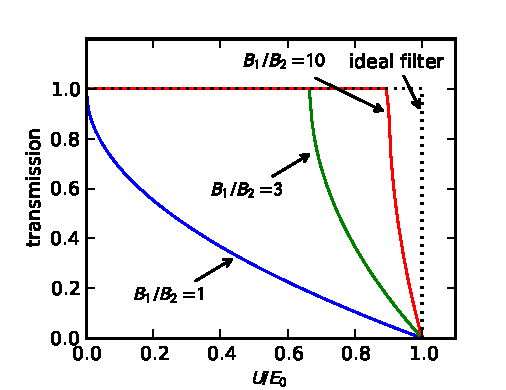
\includegraphics{gfx/mac/transmission.pdf}
}
\end{figure}
